\documentclass[main.tex]{subfiles}
\begin{document}

\section{GW detectors}

\marginpar{Monday\\ 2021-11-22}

The basic design of a GW detector is that found in \textcite[fig.\ 3]{ligoscientificcollaborationandvirgocollaborationObservationGravitationalWaves2016}. 

It is roughly a Michelson-Morley interferometer, with \SI{10}{kW} coming in
from a power-recycling mirror 
plus a Fabry-Perot cavity amplifying that power to \SI{100}{kW}. 

These cavities are roughly \SI{3}{km} long. 

The frequency of the laser is on the order of \(f \sim \SI{e15}{Hz}\), 
and it has a small dispersion in frequency space. 

What then happens is that when the length of the cavities is perturbed,
some power in each cavity is shifted into the \emph{sidebands} 
\(f_0 \pm \Delta f\) of the carrier frequency \(f_0 \), 
where \(\Delta f = f _{\text{GW}} \ll f_0 \).

We can fully control the length of the arms, 
to get our preferred interference condition. 

What can happen to laser light? It can be dissipated, 
it can come back to the mirror, but we need a device
to dump the beam and prevent it from coming back to the laser. 

A DC offset: we want a small fraction of the light, roughly \SI{.1}{\percent}, 
to get to the photodetector. 
We add a bit of the laser light to the sidebands. 

This is a homodyne detection scheme, and the laser is called a local oscillator. 

Correlated signals go back to the power recycling mirror, while
anticorrelated signals go to the detector. 

\begin{figure}[ht]
\centering
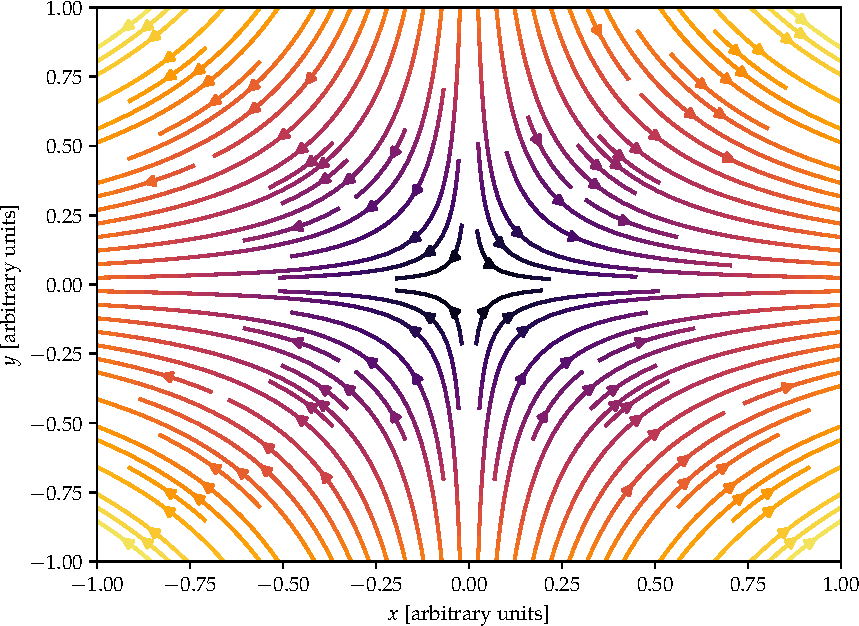
\includegraphics[width=\textwidth]{figures/polarization}
\caption{The effect of the \(h_+\) polarization of gravitational waves. Color indicates the magnitude of the field (weaker in the middle).}
\label{fig:polarization}
\end{figure}

\subsection{Noise sources}

The main \emph{environmental} noise sources are
\begin{enumerate}
    \item scattered light;
    \item seismic / vibrational noise;
    \item Newtonian noise;
    \item electromagnetic noise.
\end{enumerate}

Basically all GW detectors have a strain sensitivity curve, which is roughly 
speaking the noise referred to the quantity ``strain'': \(h = 2 \Delta L / L\). 
The ``bucket'' is centered around \SI{100}{Hz}.

The true signal we measure is the current from the photodiode. 
The noise in the detector could be reported in Ampères, but plotting 
things in this way allows us to include the response. 

A rough way to say this is 
%
\begin{align}
\text{sensitivity} = \frac{\text{noise}}{\text{response}}
\,.
\end{align}

The laser is tuned to the resonant frequency of the cavity, 
but the same does not hold for the sidebands, which are therefore not 
amplified to the same amount!

However, we can do resonant amplification of the sideband signal as well! 

There are around a hundred different relevant noise sources. 
There are ``fundamental'' noises and ``technical'' noises.
The former are a limit set by the detector configuration, nothing can be done about them. 
The technical noises can be gradually reduced by the crew working on the detector.

At high frequencies, the problem is quantum noise; 
at mid-low frequencies we have thermal noise, 
while at low frequencies the dominant contribution is environmental noise. 

Isolation from the environment means: 
\begin{enumerate}
    \item seismic isolation;
    \item reducing susceptibility to EM fields;
    \item picking a quiet environment;
    \item dealing with scattered light;
    \item vacuum system.
\end{enumerate}

Building underground helps! The seismic fields are quieter there, and
there is more insulation. 

Why do we need to build an interferometer in Europe? We (Europeans) have optical telescopes in Chile, for example. 

Telescopes only need a small amount of people to man them, 
while GW interferometers need tens of people, and not that many people want to work in an extremely remote location.

We only want the zeroth-order, Gaussian mode in the spatial 
cross-section of the decomposition of the beam. 

However, since the mirrors are not perfectly spherical higher modes
are also excited, with magnitudes of the order of \SI{20}{ppm}. 
Out of the fraction, then, a tiny fraction scatters on the edge of the 
vacuum tube (\SI{10}{ppm}) and re-enters the beam.
The vacuum tube is not seismically isolated! 
This means that that light picks up a huge amount of noise. 

We therefore need to insert a \emph{baffle}, which 
absorbs any light which hits it. 
What people now do is make detailed models of the system, 
use raytracers to figure out where the light is going 
and block it. 
People have also though about just coating the whole interior --- then, the issue becomes maintenance and coating lifetime.

Thermal noise: it is mainly about thermal vibrations of 
our suspensions, our mirrors (coating and substrate), and the electronics.

Changing the mirror's thermal noise is hard, 
electronics could be made superconductive\dots

Quantum noise is quite simple: it has only two components, 
\begin{enumerate}
    \item shot noise;
    \item radiation pressure noise.
\end{enumerate}

Once we know how the fluctuations enter our system, we can control them! 
What defines the quantum state of the detector? 

The scaling of the high-frequency part is mostly shot noise, RP noise has a lower frequency, and we can currently manage to make it negligible.

There are methods to manipulate quantum states in order to reduce quantum noise. 
The broad topic here is ``quantum nondemolition techniques''. 

There are all kinds of other noises which enter our system, but the most important ones are the ones we mentioned. 

How do we cool our experiment? 
We have roughly \SI{.5}{ppm} absorption, which means about a Watt of power going to the optics! 
A thermal link is dangerous, since it can introduce 
vibrations. 
Voyager wants to do radiative cooling, since it introduces no extra vibrations. 
However, getting to very low temperatures is basically impossible because of the \(\sim T^{4}\) temperature. 

So, ET needs a thermal link to get to \SI{10}{K} to \SI{20}{K}. 
Maybe superfluid helium could work for this purpose\dots

\subsection{Timeseries analysis}

The basic tenet of timeseries analysis is to work with the spectral representation of the data. 

This timeseries will typically be uniformly sampled. 

We define the autocorrelation as 
%
\begin{align}
C(y; t, t') = \expval{y(t) y(t')}
\,,
\end{align}
%
where the brackets denote an ensemble average.
If the noise is stationary, this will just be a function of \(\tau = t' - t\), so we get \(C(y; \tau ) = \expval{y(t) y(t + \tau )}\).

Even things like thermal and quantum noise are not really stationary, while environmental noise is \emph{definitely} not stationary. 

Fourier transforms diverge for infinitely-extending timeseries, but we can take an alternative approach, which is consistent with the fact that our signals are finite in time. 

We can only transform a section of length \(T\); its transform will be \(\widetilde{y}_T(f)\).
In the case of stationary noise, we can define the single-sided Power Spectral Density as 
%
\begin{align}
\text{PSD}(f) = S(f) = \lim_{T \to \infty} \frac{1}{T} \abs{\widetilde{y}_T(f)}
\,.
\end{align}

This converges for stationary noise. 
We can also include a 2 in the definition, it is a matter of convention.  
This is the standard way to represent timeseries in the frequency domain. 

In terms of units, \([\widetilde{y}] = [y] / \text{frequency}\); therefore, \([S] = [y]^2 / \text{frequency}\). 

If we plot \(\sqrt{S}\), this will have units of \([\sqrt{S}] = [y] / \sqrt{\text{Hz}}\). 

The integral of the PSD over all frequencies yields 
%
\begin{align}
\int_{- \infty }^{\infty } \dd{f} S(f) 
&= \lim_{T \to \infty } 
\frac{1}{T}
\int_{- T/2}^{T/2} \dd{t} y_T(t) 
\int_{- T/2}^{T/2} \dd{t'} y_T(t') 
\underbrace{\int_{- \infty }^{\infty } \dd{f} e^{2 \pi i (t - t') f}}_{ \delta (t - t')}  \\
&= \lim_{T \to \infty }
\frac{1}{T}
\int_{- T/2}^{T/2} \dd{t} y_T^2(t) = \expval{y^2} = \sigma^2_y 
\,.
\end{align}

We can also compute a \emph{bandlimited} variance: 
%
\begin{align}
\sigma^2 _{\text{bandlimited}} = \int_{f_1 }^{f_2 } \dd{f} S (f)
\,.
\end{align}

\end{document}
